\subsection{Prof. Dr. Peter Ludes}

\vspace{0.3cm}
\textbf{Main Research Interests}\\[-0.25cm]
\begin{enumerate}
\item[$\bullet$]	Mass Communication and Media Sociology, esp. Visual Communication
\item[$\bullet$]	Intercultural Comparisons
\item[$\bullet$]	Neglected News
\item[$\bullet$]	Sociology of Knowledge, Emotions, Time, Alternatives
\item[$\bullet$]	Theories of Civilizing Processes, Network Societies and Multiple Globalizations
\end{enumerate}


\vspace{0.6cm}
\textbf{Research Activities}\\[-0.25cm]

In 2006 Peter Ludes engaged (a) in the transdisciplinary study of media key visuals: The "flows of messages and images", which Manuel Castells saw as the "basic thread of our social structure", implying that "image-making is power-making", are seldom focused upon. Castells' theory of the "network society" therefore requires visual networks as illustrated by TV annual reviews of 2003-05;\\
\begin{figure}[ht]
  \begin{center}
    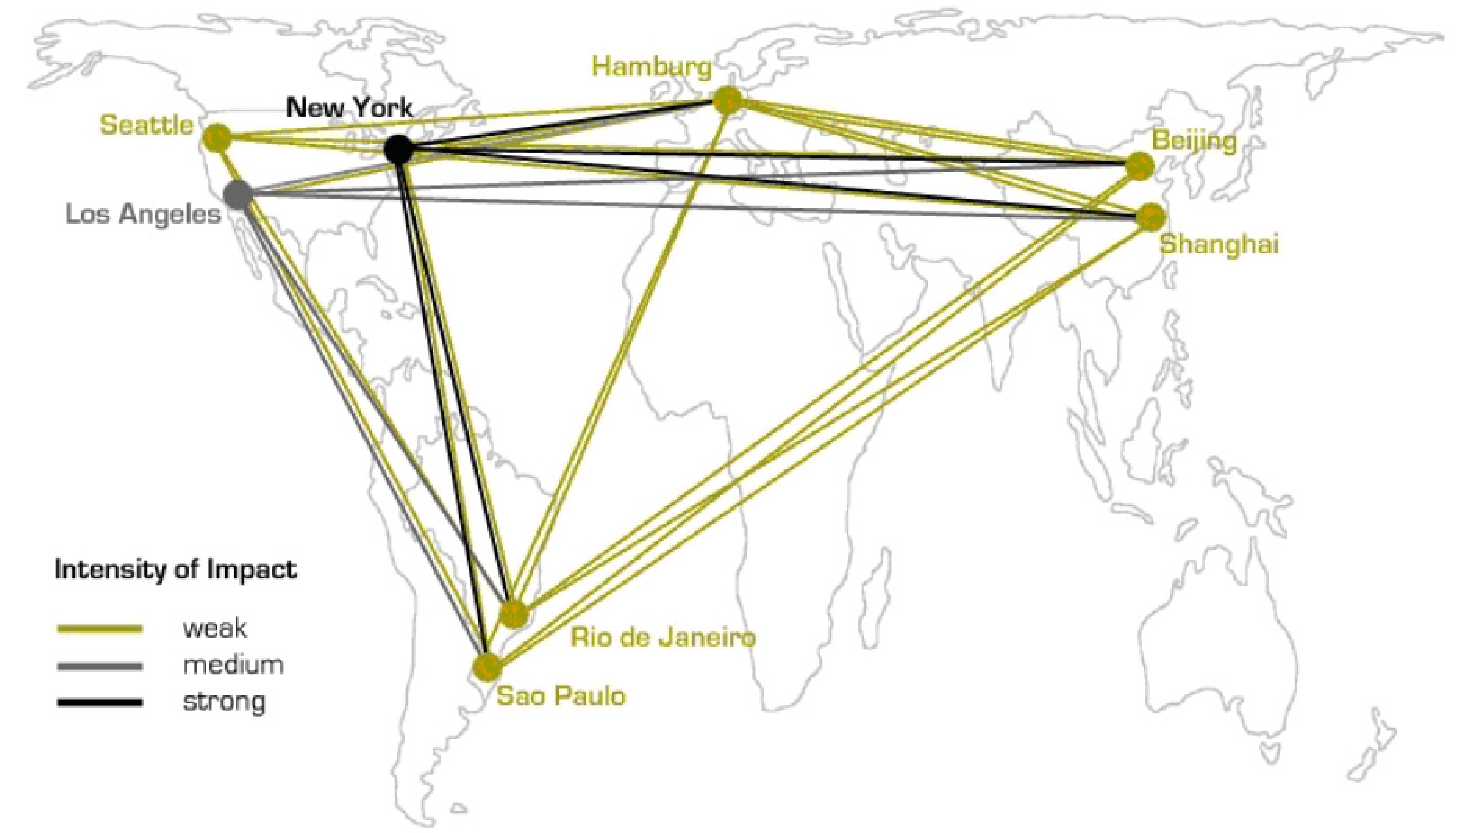
\includegraphics[width=\linewidth]{./SocSci/Ludes-fig001.pdf}
%   \mycaption{ xxx )}\label{fig:profxxx}
   \end{center}
\end{figure} 


(b) as deputy chair of the Research Network "Mass Media and Communication" of the European Sociological Association, current research on the interdependencies of techno-economic, political, and cultural developments with media formatting and contents was discussed in our e-mail network and at our conference in November 2006;
\newpage
\begin{figure}[ht]
  \begin{center}
    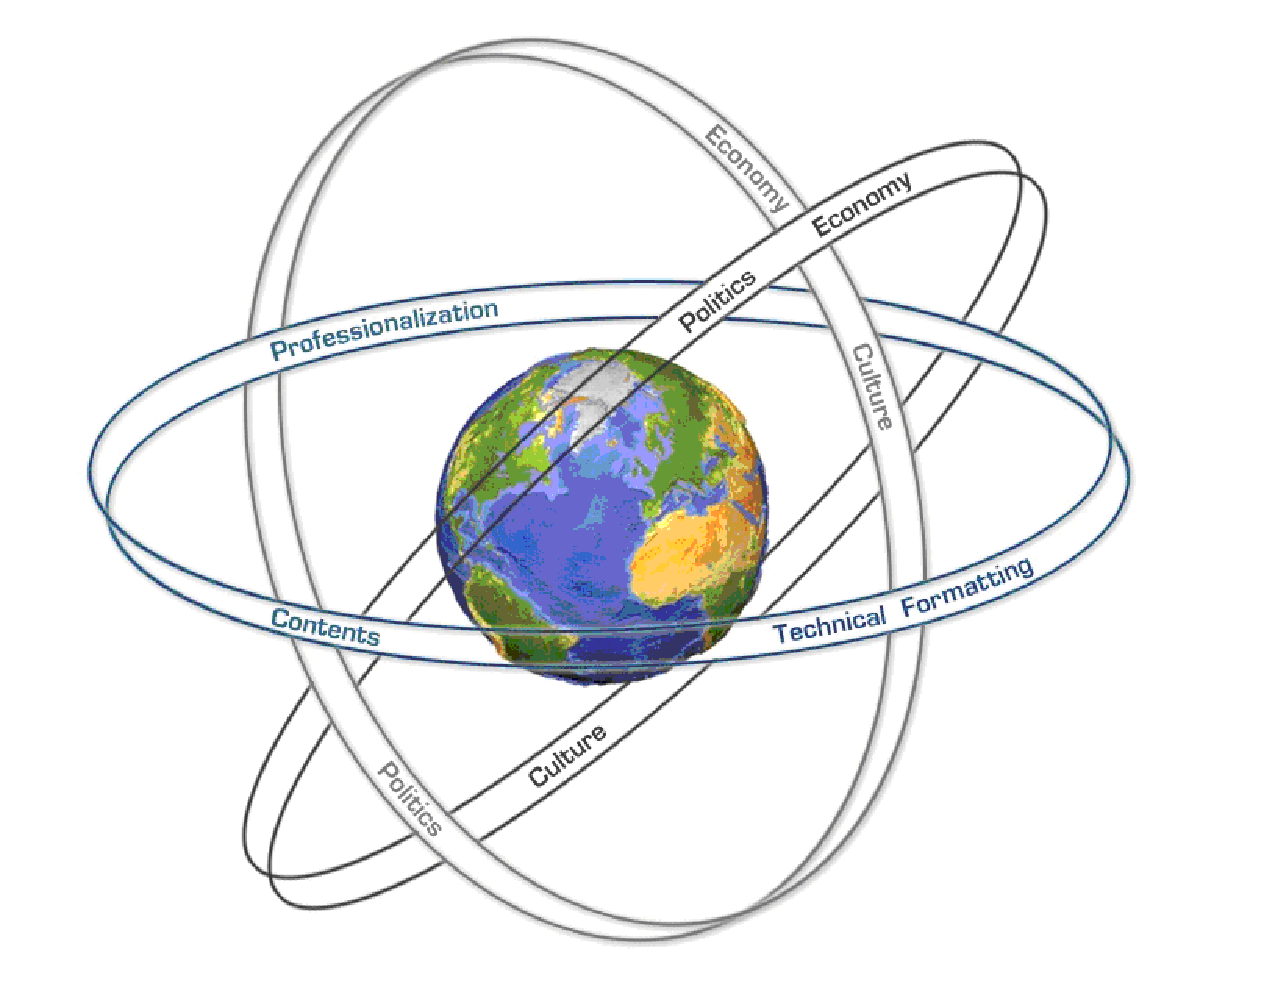
\includegraphics[width=0.8\linewidth]{./SocSci/Ludes-fig002.pdf}
%   \mycaption{ xxx )}\label{fig:profxxx}
   \end{center}
\end{figure}

(c) in the initiative "News Enlightenment" on neglected news in Germany, which he had founded in 1997, published the most neglected news of 2005 in February 2006 and has recruited new members for its jury.


\vspace{0.6cm}
\textbf{Organization of Scientific Conferences}\\[-0.25cm]
\begin{enumerate}
\item[$\bullet$]	January 2006\newline
International University Bremen\newline
Modelling and Decoding of Key Visuals in Intercultural Comparisons\newline
funded by IUB\\[-0.15cm]

\item[$\bullet$]	November 2006\newline
Antalya, Turkey\newline
Current Research\newline
funded by the European Sociological Association's Mass Media and Communications Research Network and Ankara University\newline
international participants: 15
\end{enumerate}


\vspace{0.6cm}
\textbf{Other Professional Activities}\\[-0.25cm]
\begin{enumerate}
\item[$\bullet$]	Deputy chair of the Research Network "Mass Media and Communications" of the European Sociological Association
\item[$\bullet$]	Speaker of an international group of researchers on Key Visuals
\item[$\bullet$]	Member of the task force of the International Communication Association on quality assessment
\item[$\bullet$]	External expert for the proposal for a Centre of Excellence in the Study of Democracy and the Digitisation of Audiovisual Culture (DIGICULT) of the University of Bergen
\item[$\bullet$]	Cooperation Partner for a Research Project on "Key Measures" of Prof. Dr. Leonardo Boccia, Federal University of Bahia, Salvador da Bahia, Brazil
\item[$\bullet$]	Member of the Jury of the Initiative Nachrichtenaufkl�rung \newline (www.nachrichtenaufklaerung.de) 
\item[$\bullet$]	Member of the Competence Center MultiMedia of the universities in Bremen state
\item[$\bullet$]	Referee for UK Economic and Social Research Council
\item[$\bullet$]	Member of the Research Development Committee of IUB
\end{enumerate}


\vspace{0.6cm}
\textbf{Research Personnel}\\[-0.25cm]

Christoph Kl�tsch\newline
Multimedia Research Fellow

\vspace{0.6cm}
\textbf{Guests}\\[-0.25cm]

Dr. Leonardo Boccia, Professor of Scenic Arts and Cultural Studies, Federal University of Salvador da Bahia (UFBA), funded by UFBA


